\documentclass[11pt,a4paper]{article}

% --- Packages Included ---
\usepackage[utf8]{inputenc}
\usepackage{amsmath, amssymb, amsthm}
\usepackage{float}
\usepackage{tcolorbox}
\usepackage{geometry}
\usepackage{graphicx}
\usepackage{tikz}
\usepackage[colorlinks=true, 
            linkcolor=black, 
            urlcolor=black, 
            citecolor=black]{hyperref}

\geometry{margin=2.5cm}

% --- Title and Author ---
\title{\textbf{The RSA Cryptosystem: A Mathematical Perspective}}
\author{Nenad Jakovchevski}
\date{\today}

% --- Theorem Environment Setup ---
\newtheorem{theorem}{Theorem}[section]
\newtheorem{lemma}[theorem]{Lemma}
\newtheorem{definition}[theorem]{Definition}
\newtheorem{example}{Example}
\numberwithin{equation}{section}

% --- New Environment: Custom Algorithm Box ---
\newenvironment{algorithmBox}[1][]
{
    \begin{tcolorbox}[
        colback=gray!10,              % Background color: LIGHT GRAY
        colframe=gray!50!black,       % Border: DARK GRAY
        sharp corners,                % Corners: Sharp
        boxrule=0.5pt,                % Border thickness: Not much
        left=5pt, right=5pt,          % Horizontal padding
        top=5pt, bottom=5pt,          % Vertical padding
        title={\centering\bfseries RSA Cryptosystem}, % Constant Title
        fonttitle=\small\sffamily,    % Title font: small, sans-serif
        #1                            % Optional Argument for customizing
    ]
    \begin{minipage}{\linewidth}     % Ensures content wraps within the box
}
{
    \end{minipage}
    \end{tcolorbox}
}

\begin{document}

% --- START of Leadng Page ---

\maketitle

\thispagestyle{empty}

\vspace{1cm}

\tableofcontents

\vspace{1cm}

\listoffigures

% --- END of Leading Page ---
\newpage
% --- START of Section 1: Introduction ---

\pagenumbering{arabic}
\pagestyle{plain}
\section{Introduction}
\hspace{0.5cm} The protection of information transmitted across increasingly digital landscapes is not just pivotal, it is imperative. This necessity gives rise to the field of cryptography, a discipline as ancient as it is essential in our modern world. From ancient Spartans who used an early transposition cipher to scramble the order of the letters in their military communication, to modern cryptography since the 1970s for online banking to private messaging, the confidentiality and authenticity of data transmission has always been crucial \cite{dasGold}.

Among the most influential achievements in the field is the \textbf{RSA} cryptosystem, named after its inventors Ron \textbf{R}ivest, Adi \textbf{S}hamir, and Leonard \textbf{A}dleman. This algorithm revolutionized cryptography by introducing the first practical implementation of public-key encryption, eliminating the need for pre-shared secret keys that had long constrained symmetric cryptographic systems. By solving this fundamental key distribution problem, RSA enabled secure communication in open networks and laid the foundation for modern internet security. First published in 1977, RSA remains indispensable to present security infrastructure, forming the backbone of critical protocols including HTTPS for secure web transactions, digital signature schemes for authentication, secure email through PGP\footnote{Abbreviation of Pretty Good Privacy, this is an encryption program providing cryptographic privacy and authentication.}, and certificate-based public key infrastructure.

This article focuses on the mathematical understanding and operational principles of the RSA Cryptosystem, emphasizing its reliance on number theory and computational complexity for security. By analyzing the RSA mechanism, the aim is to obtain a clear understanding of both its theoretical foundation and practical implementation, providing a resource that is as informative as it is accessible to those interested in the field.

\textbf{Organization of the Paper.}The remainder of this paper is structured as follows to facilitate a comprehensive examination of the RSA Cryptosystem:
\begin{enumerate}
    \item Section 2 explores the mathematical groundwork necessary for understanding RSA, including prime numbers and modular arithmetic.
    \item Section 3 details the RSA algorithm itself, covering key generation, with the encryption and decryption processes.
    \item Section 4 addresses the correctness of RSA, offering a proof to validate the encryption and decryption operations.
    \item Section 5 discusses the security aspects of RSA, analyzing potential vulnerabilities, and reviewing the cryptosystem’s applications in real-world scenarios.
    \item Finally, Section 6 concludes the paper with a summary of the findings and reflections on the future of RSA in the evolving landscape of cryptography.
\end{enumerate}

% --- END of Section 1: Introduction ---
\newpage
% --- START of Section 2: Mathematical Background ---

\section{Mathematical Background}
The security of the RSA cryptosystem rests on the mathematical concepts from number theory. Three principles form its core: the properties of prime numbers, the arithmetic of modular systems, and Euler's insights about relative primes. These elements combine to create the one-way functions that make RSA both functional and secure.
\subsection{Prime Numbers in Cryptographic Systems}
\begin{definition} A \textbf{prime number} is an integer greater than 1 that has no positive divisors other than 1 and itself. \end{definition}
\noindent The security of RSA encryption fundamentally relies on properties of prime numbers, which are used for its key generation process. These special integers have fascinated mathematicians for a long time due to their unique properties and distribution within the number system. 
In the context of RSA cryptography, primes play several critical roles:
\begin{itemize}
\item They enable the creation of products of two large primes that are computationally difficult to factor.
\item The uncommonness of large primes provides security through computational complexity.
\item Their use in Euler's totient function establishes the foundation for key generation.
\end{itemize}
The security of RSA specifically relies on this imbalance between the ease of multiplying two large primes and the extreme difficulty of factoring their product. This one-way function property makes primes ideal for cryptographic applications, as recognizing primes is computationally feasible (via tests like Miller-Rabin), while factoring their products remains intractable for classical computers when sufficiently large primes are chosen (typically 1024-bit or larger in modern implementations).

\subsection{Modular Arithmetic in RSA}
Having established the fundamental role of prime numbers in RSA's foundation, we now examine the arithmetic framework that enables their cryptographic application. Modular arithmetic provides the mathematical structure that transforms prime-based constructions into practical cryptographic operations.

\begin{definition}
For integers $a$, $b$, and positive integer $n$, we say $a \equiv b \pmod{n}$ if and only if $n$ divides $(a - b)$.
\end{definition}
\noindent Modular arithmetic provides the essential mathematical machinery that makes the cryptosystem operational. This "clock arithmetic" forms the basis for all computations in RSA, from key generation to message encryption and decryption in the RSA algorithm.The power of modular arithmetic in cryptography stems from several key properties:

\begin{itemize}
    \item \textbf{Closure}: Operations performed modulo $n$ always yield results within the finite ring $\mathbb{Z}/n\mathbb{Z} = \{0,1,\ldots,n-1\}$
    \item \textbf{Computational tractability}: Modular exponentiation can be efficiently computed using algorithms like the square-and-multiply method in $O(\log k)$ operations for $a^k \pmod{n}$
    \item \textbf{One-way functionality}: While computing $a^k \pmod{n}$ is efficient, extracting $k$ from $(a, a^k \bmod n)$ constitutes the discrete logarithm problem, making it computationally hard.
\end{itemize}

\newpage

\noindent The properties we've seen in modular arithmetic - particularly its \textit{wrap-around} behavior and \textit{finite field} structure - lead us to a profound result that carries modern cryptography. Consider these key observations about multiplication modulo a prime $p$:

\begin{itemize}
    \item Every number $a$ not divisible by $p$ has a multiplicative inverse.
    \item Multiplying by $a$ shuffles the numbers $\{1,2,...,p-1\}$ (forming a group under multiplication)
\end{itemize}
These properties can be seen in:

\subsubsection{Fermat's Little Theorem}

\begin{theorem}[Fermat's Little Theorem]
Let $p$ be a prime number and $a$ be an integer such that $p \nmid a$. Then
\begin{equation}\label{eq:fermat}
a^{p-1} \equiv 1 \pmod{p}
\end{equation}
\end{theorem}

\begin{proof}
First look at a list of numbers
\[ a, 2a, 3a, \ldots, (p-1)a \quad \text{reduced modulo } p. \]
We first show that these $p-1$ numbers are all different modulo $p$. Suppose, for the sake of contradiction, that we have two numbers from the list $ja$ and $ka$ such that
\[ ja \equiv ka \pmod{p}, \quad \text{so that} \quad (j-k)a \equiv 0 \pmod{p}. \]
Since $p \nmid a$, we must have $p \mid (j-k)$, but $-(p-2) \leq j-k \leq p-2$, hence $j-k = 0$, and we prove the assumption that these numbers in the list are all different.

\noindent Now to prove the theorem, we multiply all the numbers in the list together and reduce modulo $p$, which gives
\[ a \cdot 2a \cdot 3a \cdots (p-1)a \equiv 1 \cdot 2 \cdot 3 \cdots (p-1) \pmod{p}. \]
This can also be written as
\[ a^{p-1} \cdot (p-1)! \equiv (p-1)! \pmod{p}. \]
With $p \nmid (p-1)!$, we can cancel $(p-1)!$ from both sides, which gives us
\[ a^{p-1} \equiv 1 \pmod{p}, \]
and we have completed the proof of Fermat's little theorem \cite{honglin}.
\end{proof}
\noindent This theorem (Equation~\ref{eq:fermat}) is crucial for RSA because it establishes the cyclic behavior of exponents modulo $p$, which enables:
\begin{itemize}
    \item The existence of multiplicative inverses (for the decryption process).
    \item The foundation for Euler's generalization to composite modules.
    \item The "trapdoor" property of RSA's one-way function.
\end{itemize}
In particular, Fermat's theorem enables the critical step where: $m^{ed} \equiv m \pmod{n}$ for properly chosen exponents $e$ and $d$. This guarantees encrypted messages can always be recovered - a result we'll examine in detail when analyzing RSA's correctness.

% --- END of Section 2: Mathematical Background ---
\newpage 
% --- START of Section 3: The RSA Algorithm ---

\section{The RSA Algorithm}
\hspace{0.5cm} The RSA cryptosystem transforms elementary number theory into a practical encryption scheme through three deterministic operations. First, a key pair is generated by selecting two large prime numbers and computing their arithmetic derivatives. Next, plaintext messages are encrypted via modular exponentiation using publicly known parameters. Finally, ciphertext decryption applies the same mathematical operation with a privately held exponent. The scheme's security relies entirely on the computational asymmetry between integer factorization and testing of primes, while generating an RSA modulus requires a single multiplication, recovering its prime factors demands sub-exponential time for properly sized parameters.
\\


\begin{definition}[Euler's Totient Function]
The Euler totient function $\varphi(n)$ counts the number of integers between 1 and $n$ that are coprime to $n$.
\end{definition}
\begin{lemma}[Totient of Semiprimes]\label{lem:totient-semiprime}
For two distinct primes \( p \) and \( q \), their product \( n = pq \) (called a \emph{semiprime}\footnote{A semiprime is the product of exactly two prime numbers, not necessarily distinct. In RSA, we always use \emph{distinct} primes to ensure $\varphi(n) = (p-1)(q-1)$.}) satisfies:
\[\varphi(n) = (p-1)(q-1)\]
\end{lemma}

\begin{proof}
\textit{WLOG} we take that $p$  and  $q$ are distinct primes, so that there are  $pq$ total integers in $\{1,\ldots,pq\}$. Therefore, we have exactly $q$ multiples of $p$ and $p$ multiples of $q$, meaning that only $pq$ itself is a multiple of both. \\
    By inclusion-exclusion: $\varphi(pq) = pq - p - q + 1 = (p-1)(q-1)$
\end{proof}

\subsection{Key Generation}
The security of RSA begins with proper key generation, establishing secure communication without prior key exchange. The RSA key generation leverages Lemma~\ref{lem:totient-semiprime} through:
\begin{algorithmBox}
    \begin{center}
        Select large distinct primes $p$ and $q$ \\
        Compute modulus $n = p \cdot q$ \\
        Calculate $\varphi(n) = (p-1)(q-1)$ \\
        Choose encryption exponent $e$ such that: \\
         $1 < e < \varphi(n)$, \hspace{0.2cm} $\gcd(e, \varphi(n)) = 1$ \\
        Compute decryption exponent $d \equiv e^{-1} \pmod{\varphi(n)}$ \\
        \textbf{Output key pairs}:
        \textbf{Public key}: $(n, e)$,
        \textbf{Private key}: $(n, d)$
    \end{center}
\end{algorithmBox}

\subsection{Encryption Process}
With the key pair generated, encryption proceeds as follows:

\begin{algorithmBox}
    \begin{center}
        \textbf{Input}: Plaintext message $m$ where $0 \leq m < n$ \\
        \textbf{Process}: Compute ciphertext $c \equiv m^e \pmod{n}$ \\
        \textbf{Output}: Encrypted ciphertext $c$
    \end{center}
\end{algorithmBox}

\newpage 

\subsection{Decryption Process}
The private key holder can recover the original message:

\begin{algorithmBox}
    \begin{center}
        \textbf{Input}: Ciphertext $c$ \\
        \textbf{Process}: Compute plaintext $m \equiv c^d \pmod{n}$ \\
        \textbf{Output}: Original message $m$
    \end{center}
\end{algorithmBox}

\subsection{Example RSA Communication Between Alice and Bob}

Let us examine a complete secure communication scenario using RSA, where Alice needs to send Bob a confidential message. This example will illustrate the entire process from key generation to message recovery, with particular attention to the mathematical foundations that make RSA secure.

\begin{example}
\label{ex:alice-bob-rsa}
Alice wants to send Bob the single-character message "A" securely over an insecure channel. To accomplish this, they will use the RSA cryptosystem. Bob must first establish his cryptographic keys through the following procedure: \\
\textbf{Key Generation Phase:} \\
Bob begins by selecting two large prime numbers. For this demonstration, we'll use manageable primes:
\[ \textit{First prime: } p = 61, \textit{ Second prime: } q = 53 \]
He then computes the RSA modulus $n$, which serves as the first part of both his public and private keys:
\[n = p \cdot q = 61 \cdot 53 = 3233\]
Next, Bob calculates Euler's totient function for these primes:
\[\varphi(n) = (p-1)(q-1) = 60 \cdot 52 = 3120\]
For the public exponent $e$, Bob chooses a number coprime with $\varphi(n)$. A common choice is $e = 17$, which satisfies $\gcd(17, 3120) = 1$. The critical step comes in computing the private exponent $d$ as the modular inverse of $e$ modulo $\varphi(n)$. This requires solving:
\[17d \equiv 1 \pmod{3120}\]
Using the Extended Euclidean Algorithm, we find:
\begin{align*}
3120 &= 183 \cdot 17 + 9 \\
17 &= 1 \cdot 9 + 8 \\
9 &= 1 \cdot 8 + \boxed{1} \quad \text{(GCD reached)} \\
8 &= 8 \cdot 1 + 0
\end{align*}
Working backwards to express 1 as a combination of 17 and 3120:
\begin{align*}
1 &= 9 - 1 \cdot 8 \\
  &= 9 - 1 \cdot (17 - 1 \cdot 9) \\
  &= 2 \cdot 9 - 1 \cdot 17 \\
  &= 2 \cdot (3120 - 183 \cdot 17) - 1 \cdot 17 \\
  &= 2 \cdot 3120 - 367 \cdot 17
\end{align*}
Thus, the multiplicative inverse is:
\[d \equiv -367 \pmod{3120} \equiv 2753 \pmod{3120}\]
Bob now has his complete key pair:
\[ \textbf{Public key}: (n, e) = (3233, 17) \textbf{ and Private key}: (n, d) = (3233, 2753) \]
\textbf{Encryption Phase:} \\
Alice is able to obtain Bob's public key $(3233, 17)$. She converts her message "A" to its ASCII numerical representation $m = 65$. The encryption process involves computing:
\[c \equiv m^e \pmod{n} \equiv 65^{17} \pmod{3233}\]
Using the square-and-multiply algorithm for efficient computation:
\begin{align*}
65^1 &\equiv 65 \pmod{3233} \\
65^2 &\equiv 4225 \equiv 992 \pmod{3233} \\
65^4 &\equiv 992^2 \equiv 984064 \equiv 2659 \pmod{3233} \\
65^8 &\equiv 2659^2 \equiv 7070281 \equiv 611 \pmod{3233} \\
65^{16} &\equiv 611^2 \equiv 373321 \equiv 2297 \pmod{3233} \\
65^{17} &\equiv 2297 \cdot 65 \equiv 149305 \equiv 2790 \pmod{3233}
\end{align*}
The resulting ciphertext is $c = 2790$, which Alice sends to Bob.\\
\textbf{Decryption Phase:} \\
Upon receiving $c = 2790$, Bob uses his private key $(3233, 2753)$ to decrypt it:
\[m \equiv c^d \pmod{n} \equiv 2790^{2753} \pmod{3233}\]
While the full computation of $2790^{2753}$ is extensive, we can verify the result using Euler's theorem. Since $2753 \times 17 \equiv 1 \pmod{3120}$:
\[
2790^{2753} \equiv (65^{17})^{2753} \equiv 65^{17 \cdot 2753} \equiv 65^{1 + k\cdot 3120} \equiv 65 \cdot (65^{3120})^k \equiv 65 \cdot 1^k \equiv 65 \pmod{3233}
\]
The decrypted message $m = 65$ correctly corresponds to the ASCII character "A", completing the secure transmission.
\end{example}

\begin{table}[H]
\centering
\label{tab:rsa-workflow}
\begin{tabular}{|l|l|}
\hline
\textbf{Component} & \textbf{Value} \\ \hline
Selected Primes & $p=61$, $q=53$ \\ \hline
RSA Modulus & $n=3233$ \\ \hline
Totient Value & $\varphi(n)=3120$ \\ \hline
Public Exponent & $e=17$ \\ \hline
Private Exponent & $d=2753$ \\ \hline
Original Message & $m=65$ (ASCII "A") \\ \hline
Encrypted Ciphertext & $c=2790$ \\ \hline
Decrypted Message & $m=65$ \\ \hline
\end{tabular}
\caption{Complete RSA Workflow Between Alice and Bob}
\end{table}

As demonstrated in Example~\ref{ex:alice-bob-rsa} and summarized in Table~\ref{tab:rsa-workflow}, the RSA cryptosystem provides a secure method for transmitting confidential information. This example, while using small numbers for clarity, perfectly illustrates the principles used in real-world implementations where the prime numbers are typically hundreds of digits long.

% --- END of Section 3: RSA Algorithm ---
\newpage 
% --- START of Section 4: RSA Correctness ---

\section{Proof of RSA Correctness}

The security of RSA relies on its mathematical foundations. Therefore, a formal proof of why the decryption process correctly recovers the original message is needed. The proof will utilize Fermat's Little Theorem and the Chinese Remainder Theorem \cite{wikiRSA}.
\begin{theorem}[RSA Correctness]
For any RSA parameters $(p, q, e, d)$ with $n = pq$ and $ed \equiv 1 \pmod{\lambda(n)}$, and any message $0 \leq m < n$:
\[(m^e)^d \equiv m \pmod{n}\]
where $\lambda(n) = \text{lcm}(p-1, q-1)$ is the Carmichael function.
\end{theorem}
\begin{proof}
The proof proceeds by showing congruence modulo $p$ and $q$ separately. \\
\noindent \textbf{Case 1: Congruence modulo $p$} \\
Since $ed \equiv 1 \pmod{\lambda(n)}$, there exists an integer $k$ such that:
\[ed = 1 + k\cdot\lambda(n)\]
Because $\lambda(n) = \text{lcm}(p-1,q-1)$, we know $p-1$ divides $\lambda(n)$, so we can write:
\[ed = 1 + t(p-1) \quad \text{for some integer } t\]
Now consider two subcases:
\begin{itemize}
\item \textbf{Subcase 1.1}: If $m \equiv 0 \pmod{p}$
\[ m^{ed} \equiv 0^{ed} \equiv 0 \equiv m \pmod{p} \]
\item \textbf{Subcase 1.2}: If $m \not\equiv 0 \pmod{p}$
\begin{align*}
m^{ed} &\equiv m^{1 + t(p-1)} \pmod{p} \\
&\equiv m \cdot (m^{p-1})^t \pmod{p} \\
&\equiv m \cdot 1^t \pmod{p} \quad \text{(by Fermat's Little Theorem)} \\
&\equiv m \pmod{p}
\end{align*}
\end{itemize}
\noindent \textbf{Case 2: Congruence modulo $q$} \\
The proof for $q$ follows identically by symmetry:
\[ed = 1 + s(q-1) \quad \text{for some integer } s \]
\begin{itemize}
\item \textbf{Subcase 2.1}: If $m \equiv 0 \pmod{q}$
\[m^{ed} \equiv 0^{ed} \equiv 0 \equiv m \pmod{q}\]
\item \textbf{Subcase 2.2}: If $m \not\equiv 0 \pmod{q}$
\begin{align*}
m^{ed} &\equiv m^{1 + s(q-1)} \pmod{q} \\
&\equiv m \cdot (m^{q-1})^s \pmod{q} \\
&\equiv m \cdot 1^s \pmod{q} \quad \text{(by Fermat's Little Theorem)} \\
&\equiv m \pmod{q}
\end{align*}
\end{itemize}
Therefore, \\
Having established that:
\[
m^{ed} \equiv m \pmod{p} \quad \text{and} \quad m^{ed} \equiv m \pmod{q}
\]
and since $p$ and $q$ are distinct primes, the Chinese Remainder Theorem guarantees:
\[ m^{ed} \equiv m \pmod{pq} \]
This completes the proof that RSA decryption correctly recovers the original message.
\end{proof}

% --- END of Section 4: RSA Correctness ---
\newpage
% --- START of Section 5: RSA Vulnerabilities and Attacks ---

\section{RSA Vulnerabilities and Attacks}
While the RSA Cryptosystem stands on a robust mathematical foundation, practical implementations can introduce vulnerabilities that may compromise its security. This section explores common attacks that exploit such weaknesses, emphasizing the importance of cautious and precise implementation practices.
\subsection{Small Exponent Attack}
A notable vulnerability arises when the public exponent $e$ is chosen to be too small. A common choice for $e$ is $65537$, but some systems, for reasons of computational efficiency, may opt for smaller values like $e=3$. This can lead to significant security flaws as illustrated below.

\begin{figure}[H]
\centering
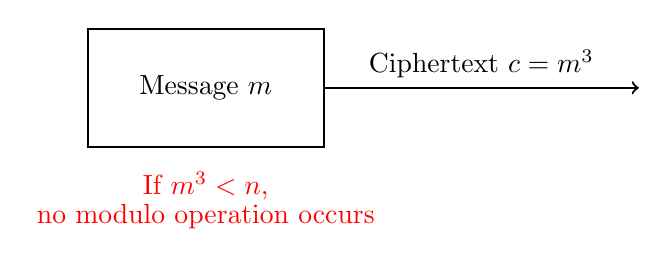
\begin{tikzpicture}
    \draw[thick] (0,0) rectangle (3,1.5);
    \node at (1.5,0.75) {Message \( m \)};
    \draw[->, thick] (3,0.75) -- (7,0.75) node[midway, above] {Ciphertext $ c = m^3$};
    \node[red, below] at (1.5,-0.2) {If $ m^3 < n $,};
    \node[red, below] at (1.5,-0.6) {no modulo operation occurs};
\end{tikzpicture}
\caption{Visualization of the Small Exponent Attack.}
\label{fig:small-exponent-attack}
\end{figure}

This visualization of Figure~\ref{fig:small-exponent-attack}  highlights the encryption process for a small message $m$ and a small exponent $e$, emphasizing the critical condition $m^3 < n$. To safeguard against this attack, cryptographers universally advocate for the use of larger public exponents in practical RSA implementations. A widely accepted choice is $e \geq 65537$, which not only mitigates the risk of such vulnerabilities but also maintains computational efficiency due to its binary representation (a small number of 1s in its binary form reduces the number of operations required during exponentiation).

\subsection{Timing Attack}
Timing attacks are a type of side-channel attack where the time taken for cryptographic operations is measured to gather secret data, such as private keys. In RSA, these attacks exploit the time it takes to perform decryption operations, which can vary based on the input data due to conditional branches in the decryption algorithm. \\
The figure below illustrates the steps involved in a timing attack against an SSL server using RSA decryption:
\begin{enumerate}
    \item The attacker sends a \textbf{ClientHello} message to initiate a connection.
    \item The server responds with a \textbf{ServerHello} message that includes its public key.
    \item The attacker measures the time $t_1$ just before sending a message designed to be decrypted by the server's private key.
    \item The server processes the request and sends an alert back to the attacker.
    \item Upon receiving the alert, the attacker records the time $t_2$.
    \item The attacker calculates the time difference $t_2 - t_1$, which provides insights into the decryption process.
\end{enumerate}

\begin{figure}[H]
\centering
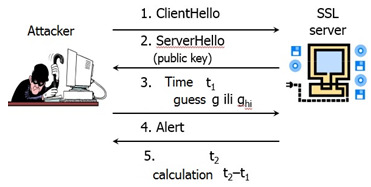
\includegraphics[width=0.7\textwidth]{timing_attack.png}
\caption{Timing attack process involving RSA decryption on an SSL server. \cite{atk}}
\label{fig:timing_attack}
\end{figure}
\noindent Figure \ref{fig:timing_attack} depicts the steps an attacker takes to measure how long it takes the server to decrypt a message. Effective countermeasures against timing attacks include implementing constant-time algorithms for cryptographic operations to ensure that they take the same amount of time to execute, regardless of the input data.

\subsection{Additional Threats to RSA Security}
Beyond the two vulnerabilities detailed above, RSA faces a variety of additional threats that can undermine its security if not properly addressed. These include:

\begin{itemize}
    \item \textbf{Factorization of Weak Modules}: The strength of RSA relies on the modulo $n$, which is the product of two large prime numbers. If $n$ is too small or if the primes are poorly chosen—such as being too close together—an attacker might successfully factor $n$ using advanced algorithms like the quadratic sieve or number field sieve. Once factored, the private key can be derived, rendering the system insecure.

    \item \textbf{Padding Oracle Attacks}: Many RSA implementations use padding schemes to ensure messages meet specific formatting requirements before encryption. However, if an implementation leaks information about padding errors (e.g., through error messages or timing differences), an attacker can exploit this as an "oracle" to decrypt messages incrementally without knowing the private key.

    \item \textbf{Side-Channel Attacks}: In addition to timing attacks, other side-channel methods—such as analyzing power consumption, electromagnetic emissions, or even acoustic signals during computation—can reveal sensitive information about the cryptographic process. These attacks exploit physical characteristics of the hardware rather than mathematical weaknesses.

    \item \textbf{Quantum Computing Threats}: The future of large-scale quantum computers poses a long-term threat to RSA. Using Shor’s algorithm, a sufficiently powerful quantum computer could factor large numbers exponentially faster than classical computers, effectively breaking RSA encryption by computing private keys from public ones.
\end{itemize}
To protect RSA-based systems from these vulnerabilities, meticulous attention to implementation details is vital. This includes focusing on the best practices such as using sufficiently large key sizes (at least 2048 bits in modern contexts) to reduce factorization attempts, selecting robust public exponents like $e = 65537$, and employing secure padding schemes and constant-time operations. Furthermore, staying informed about emerging cryptographic research and evolving attack methodologies ensures that defenses remain effective against both current and future threats.

% --- END of Section 5: RSA Vulnerabilities and Attacks ---
\newpage 
% --- START of Section 6: Conclusion ---

\section{Conclusion}
\hspace{0.5cm}This article has explored the RSA Cryptosystem in detail, explaining its mathematical foundation, operational mechanics, and potential vulnerabilities. Through detailed examination, the strengths and limitations of RSA have been highlighted, emphasizing the essential need for meticulous implementation and strong cryptographic practices.

The processes of key generation, encryption, and decryption within RSA have been detailed, with proofs provided to validate the algorithm's correctness. The exploration of various attack vectors—from side-channel attacks to quantum computing threats—underscores the multiple challenges faced in securing RSA implementations. 

RSA continues to be a key component of public key cryptography, but it faces challenges from the fast pace of technological advances, including quantum computing. It is crucial that the cryptographic community keeps innovating and researching new ways to stay ahead of these emerging threats. 

RSA is a vital part of modern cryptography, helping to secure everything from online communications to digital transactions. However, its security is not guaranteed and requires ongoing efforts to address new vulnerabilities. Moving forward, the insights gained from studying RSA will surely shape future cryptographic methods, ensuring that our digital exchanges are safe and reliable.



% --- END of Section 6: Conclusion ---
\newpage
% --- START of Bibliography ---

\begin{thebibliography}{99}

% --- USED BOOKS ---
\bibitem{stinson}
Douglas R. Stinson and Maura Paterson, 
\textit{Cryptography: Theory and Practice}. 
Fourth Edition, CRC Press, 2019.

% --- USED ARTICLES ---
\bibitem{hac}
Alfred J. Menezes, Paul C. van Oorschot, and Scott A. Vanstone, 
\textit{Handbook of Applied Cryptography}. 
CRC Press, 1996.\\
\url{http://cacr.uwaterloo.ca/hac/}

\bibitem{honglin}
Honglin Xu,
\textit{RSA as a Cryptosystem},
MIT Research High School Program, 2024.\\
\url{https://math.mit.edu/research/highschool/primes/circle/documents/2024/Honglin.pdf}

\bibitem{dasGold}
Rayan Das and Guillermo Goldsztein,
\textit{Mathematics Behind the RSA Algorithm},
Journal of Student Research, 2023.\\
doi: \href{https://doi.org/10.47611/jsrhs.v12i1.3990}{10.47611/jsrhs.v12i1.3990}

\bibitem{wikiRSA}
Wikipedia contributors,
\textit{RSA (cryptosystem)},
Wikipedia, The Free Encyclopedia. \\
\url{https://en.wikipedia.org/wiki/RSA_cryptosystem} 

\bibitem{atk}
Ćurguz and Jelena,
\textit{Vulnerabilities of the SSL/TLS Protocol},
ResearchGate 2016. \\
doi: \href{https://doi.org/10.5121/csit.2016.60620}{10.5121/csit.2016.60620}

\end{thebibliography}

% --- END of Bibliography ---

\end{document}
